\section{Research Results}
\label{sec:results}

\begin{table*}[ht]
    \centering
    \caption{Results of running the clustering algorithms on each of the code-bases.}
    \begin{tabular}{|c|c|c|c|c|c|c|}
        \hline
             \multirow{2}{*}{Library} & \multirow{2}{*}{Sub-Partitions} & One-Valued & \multicolumn{2}{c|}{Mean MQ} & \multicolumn{2}{c|}{Mean WMQ} \\
        \cline{4-7}
            & & Sub-Partitions & Gradient & Genetic & Gradient & Genetic \\
        \hline
        \hline
            UCX & 87 & 58 & 0.4425 & 0.4471 & 0.4430 & 0.4479 \\
        \hline
            OFI & 204 & 164 & 0.3738 & 0.3751 & 0.3686 & 0.3708 \\
        \hline
            Portals & 47 & 40 & 0.4471 & 0.4031 & 0.4046 & 0.4390 \\
        \hline
            %SOS & 2 & 0 & 0.4256 & 0.4396 & 0.4401 & 0.4236 \\
        %\hline
        %    OpenMPI & & & & & & \\
        %\hline
        %\hline
        %    UCT & & & & & \\
        %\hline
        %    UCP & & & & & \\
        %\hline
        %    UCS & & & & & \\
        %\hline
    \end{tabular}
    \label{tab:mq_results}
\end{table*}


\begin{figure}[Ht]
    \centering
    \begin{tabular}{c}
        \includegraphics[width=0.96\linewidth]{figures/ucx_analysis/ucp.png} \\
        a) UCP \\
        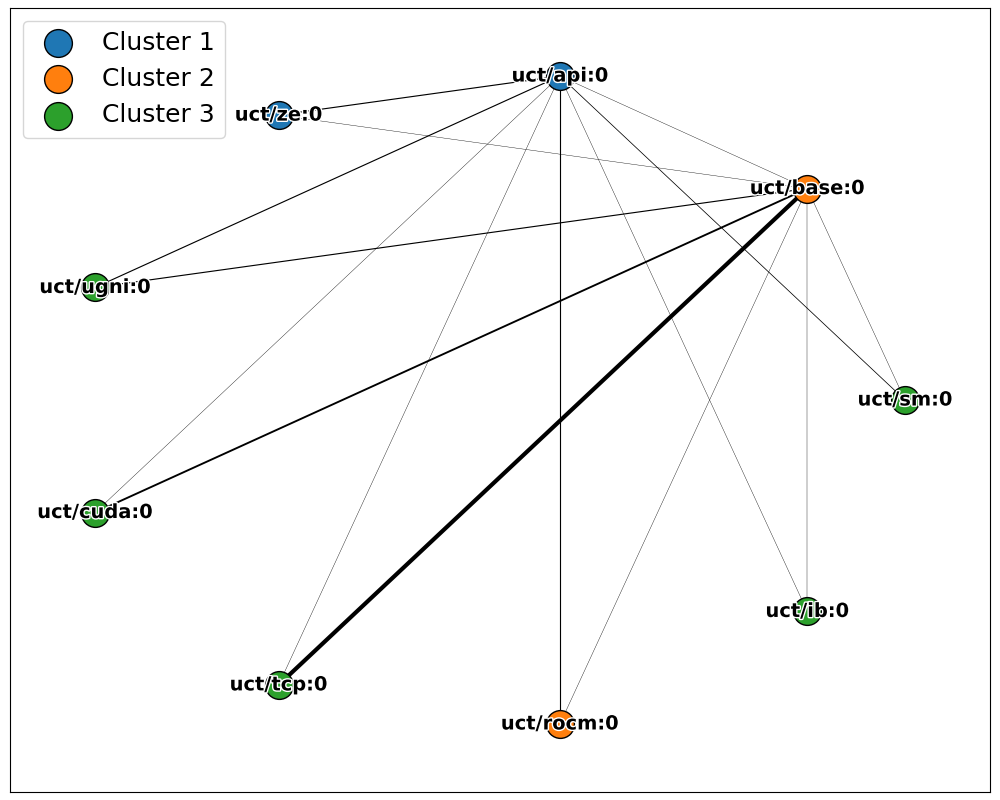
\includegraphics[width=0.96\linewidth]{figures/ucx_analysis/uct.png} \\
        b) UCT \\
        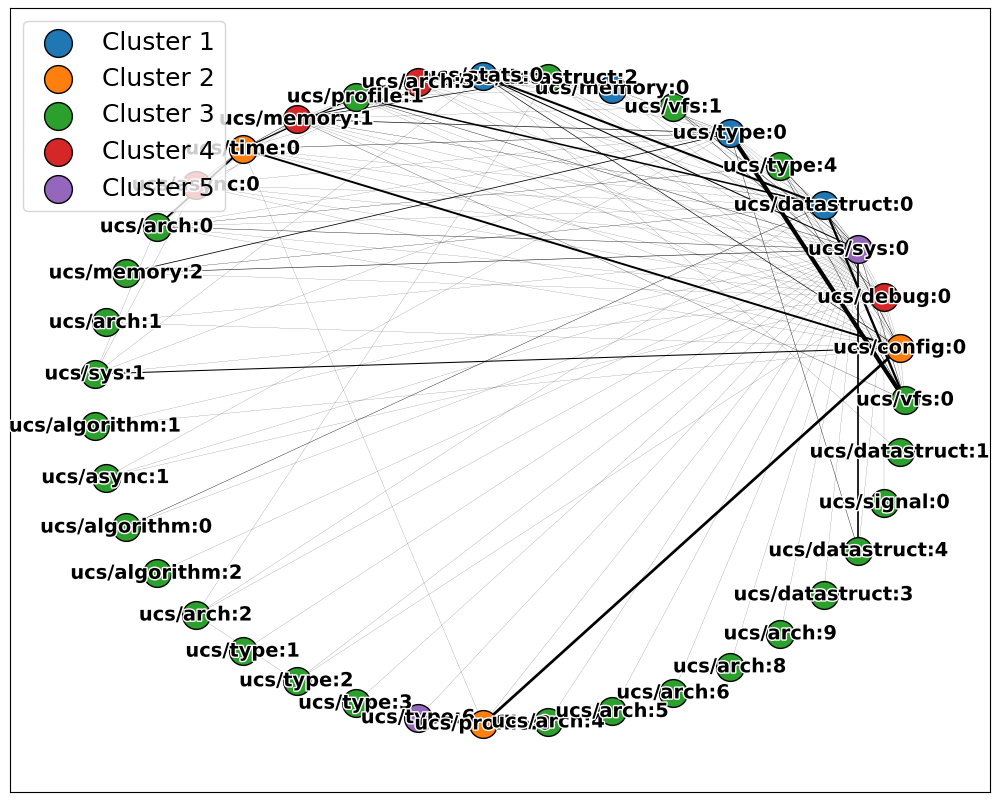
\includegraphics[width=0.96\linewidth]{figures/ucx_analysis/ucs.png} \\
        c) UCS \\
    \end{tabular}
    \caption{Network diagrams for UCX's top-level components.}
    \label{fig:ucx_components}
\end{figure}

This section seeks to answer three research questions (RQs) by analyzing the results of executing the methodology outlined in Section \ref{sec:methodology}. The research questions are:
\begin{enumerate}
    \item Which clustering algorithm results in the lowest mean MQ value across the different HPC code-bases?
    \item Are clustering algorithms useful in extracting the architecture of HPC middleware libraries?
    \item How can the information generated by the proposed methodology be used to help deepen ones understanding of UCX?
\end{enumerate}

RQ1 aims to identify the best clustering algorithm for architecture extraction and will be achieved by quantitatively testing each of the algorithms with MQ and WMQ heuristics for each of the code-bases. RQ2 looks at if the clustering results are useful in extracting architecture patterns on arbitrary HPC libraries in order to check the utility of the methodology proposed in this work. This will be done through a qualitative inspection of the hierarchical clusters that were produced through the methodology's execution on each of the code-bases. RQ3 builds on the results of RQ2 by exploring how the surface-level intuition gained about the architecture can be used to examine the source code in a more informed manner. Only UCX will be explored for RQ3 due to the depth of analysis required and space constraints.
% RQ3 aims to take a deeper dive into the utility of this methodology for developing an understanding of a code-base. 

%%%%%%%%%%%%%%%%%%%%%%%%%%%%%%%%%%%%%%%%%%%%%%%%%%%
\subsection{Algorithm Performance}
\label{subsec:alg_perf}

Both algorithms were run for each of the libraries with both the weighted and unweighted MQ variants. Table \ref{tab:mq_results} show the results of these tests with the best values from 10 random seeds. The number of sub-partitions in the table is the number of partitions that were clustered in order to build the project-level hierarchy. In the example of UCX shown in Figure \ref{fig:graph_example} d), the top level partition is composed of ucp:0, uct:0, ucs:0, and ucs:1. This would count as 4 sub-partitions at the top-level and then be run recursively to determine the sub-partition count for the entire code-base. Since the number of sub-partitions generated are deterministic based on the directory structure and fixed k values, the sub-partition counts are constant across each algorithm. For the mean values, only hierarchical clusters with non-one MQ values were considered as to not skew the results with MQ values that were deterministic rather than generated by the algorithms.

The general results seen in the table are that there is no common trend for which algorithm results in the best MQ value when looking across multiple code-bases. The differences between MQs for algorithms in any given code-bases were also marginal with the greatest difference being Portals with a $(gradient - generic)$ MQ difference of 0.0440 and a WMQ difference of -0.0344. It is an interesting point that, even looking at the MQ and WMQ heuristics for the same code-base, there isn't a consistency in the best performer between the two algorithms. This leads to the conclusion that the performance difference in finding the best MQ values between the two algorithms and the two heuristics is inconsequential. 

%%%%%%%%%%%%%%%%%%%%%%%%%%%%%%%%%%%%%%%%%%%%%%%%%%%
\subsection{Architecture Extraction}
\label{subsec:arch_extraction}

For the UCX library, the components of UCS, UCT, and UCP are heavily dependent on one another with a lot of dependencies that interweave their construction, but each of the components also has their own distinct architecture. Each of the major components of UCX are shown in Figure \ref{fig:ucx_components}, but the components of the other libraries will only be discussed and not be shown due to space restrictions. UCP is focused around its api and core components with core being fully connected to all other components and api primarily servicing the wireup and rma components. UCS is heavily dependent on its datastruct component which services data structures for in-memory processing alongside its sys component which implements the system calls for OS bypassing. UCT is built around its api and base components, similar to UCP, but each of the components only connect to these two which reflects how each component is instantiated based on what hardware is being used.

For the OFI library, the broad architecture that can be extracted from the results are that the "include" directory is where all of the *.h files that connect components are kept. The *.h files in the component directories are primarily for dependencies within the same component (e.g. rdma interface files reference other rdma files directly, but not ucx interface files). At this top level, the primary files that dictate dependencies are ofi\_util.h which bootstraps the communication protocol components and ofi\_enosys.h that connects the hardware-level interactive components such as atomic operation, network endpoint address resolutions, and message tagging.

For the Portals library, there are virtually no dependencies in the code-base. Upon further inspection from a dumping of the dependency graph data, it appears that there are a over 100 *.h files that simply point to their respective *.c files and an equally great number that don't point to any files. The majority of the *.h files that did point to a *.c file were in the runtime component which instantiated system calls. This makes sense as portals is strictly a modular network API that sits directly on IB verbs rather than providing a framework such as UCX or OFI.

Overall, the qualitative analyses of the broad graphical results have proven to be useful in the extraction of broad architectures for each of the HPC libraries. These analyses are not exhaustive of what can be extracted due to space constraints and have only considered the points that are apparent in the network diagrams. The concern with the analyses conducted is that the analytical points related to the architecture that were extracted were dependent exclusively on the dependency weightings between files rather than the automatic clustering of files done by the algorithms. The cluster results provided no helpful insight beyond what was visible in the dependency analysis and attempts at gleaming insight from them were fruitless. These results lead to the conclusion that the use of clustering algorithms were not useful in extracting the architecture of HPC middleware libraries.

%%%%%%%%%%%%%%%%%%%%%%%%%%%%%%%%%%%%%%%%%%%%%%%%%%%
\subsection{UCX Architectural Patterns}
\label{subsec:ucx_arch}

Next is to do a deep-dive into UCX to see what deeper meaning can be extracted when the results from the network diagrams are considered in conjuncture with an analysis of the source code. Starting with UCP, the core component which had a high degree of dependencies to other components was primarily due to the ucp\_ep sub-component which define the endpoint characteristics for the network. This component establishes endpoint control (e.g. instantiation, connection characteristics, protocols, etc.) which is a fundamental aspect of network communications. These files have dependencies utilize the lane protocols from the proto component and the endpoint matching from the wireup component. Further analyses revealed that ucp\_ep is indeed the backbone component for UCP's design which the other components build on top of. For example, stream, rndv, and rma are all protocols that sit on top of the endpoint connection and use core's other sub-components (e.g. workers, buffers, and requests) to execute. The API component also had a notable number of dependencies, but that's primarily due to it being the interface for usage external to UCP which necessitates its inter-dependencies to all externally visible components.

Looking next at the construction of UCS, the datastruct and sys components were prevalent in the initial analysis. The datastruct component has little-to-no internal structure that lends itself to further analysis with pseud-random connections between its sub-components, but it is worth noting that datastruct is the most commonly called component across not only UCS, but UCP and UCP as well. This makes sense as it implements all of the optimized datatypes and how they are managed directly in memory. Switching to the sys component, the sub-component by the same name (i.e. sys/sys) is the most heavily utilized. This appears to be due to it being where the system calls are primarily implemented with the other sub-components acting as supports for it. It is also worth noting that UCS doesn't have an API component unlike UCP and UCT. This makes sense as UCS has been seen here to primarily implement fundamental building blocks such as system calls and data structures which UCP and UCT can utilize rather than providing services such as the endpoint connections seen in the UCP analysis.

Finally looking at UCT, the base component immediately appears to be the backbone of the design with other components being connected to it exclusively. The API component is the notable exception to this, but due to the reasons mentioned in the UCP analysis is deemed to be not of any greater note. Looking at the base component's construction, the iface sub-component is the most utilized as it provides a template for the transport interface model that's being used by other components (i.e. cuda, ib, rocm, tcp, etc.). Further analysis revealed that this is common for the other sub-components of the core module as well as the component that is implemented depending on the target hardware drivers specified at compilation. For example, if CUDA drivers and InfiniBand are detected for hardware support then the cuda and ib components of the transport layer are built over the base template at compile time.

